\documentclass[10pt]{article}
\usepackage{icmlko}

\icmlmeta{IP 파운데이션 월드모델}{327}{위약 서른이 알려 준 바닥}{노트 326을 판에 태웠다 --- 이겼는데, 위약 서른을 돌려 보니 검출 바닥이 우리가 알던 것의 1.65배였다}

\begin{document}

\twocolumn[
\icmlheader

\begin{abstract}
노트 326이 아이돌 94행 중 68행(2025년 이전)을 학습에 넣으면 유보 순위상관이
0.2199$\to$0.4728 이라고 쟀다. 그건 \textbf{손으로 만든 부스팅}이었다.
오늘 판에 태웠다. \textbf{현행 판의 아이돌 0.2108 $\to$ 0.2831}
($+$0.0723) · \textbf{판 0.3030 $\to$ 0.3061}($+$0.0031, 미결정 폭 0.010
안) · \textbf{어느 도메인도 $2.77{\times}$짝SE 를 안 넘는다.} 배포 규칙
①② 를 다 통과한다. \textbf{그런데 노트 133이 첫 양수를 그대로 채택하지
말라고 한다.} 위약을 돌렸다 --- 추가 68행의 \emph{라벨만} 섞고 씨앗 서른.
결과가 셋이다. ① \textbf{위약 중앙 0.0923 이 같은 경로 대조 0.0969 와
사실상 같다}(위약이 대조 이상인 몫 정확히 0.500) --- \textbf{행이 늘어서
버는 몫은 판에서 0 이다.} 노트 326의 손 실험에서 위약이 이득의 30\%를
먹었던 것과 다르다. ② 진짜 0.2831 은 서른 중 하나만 넘는다 ---
\textbf{$p{=}$0.033 · $z{=}$2.13.} 이긴 게 맞다, 겨우. ③ 그리고 셋째가
제일 크다: \textbf{위약 SD 가 0.0922 인데 아이돌 짝SE 는 0.056 이다.}
노트 274가 검출 바닥을 $2{\times}$짝SE$=$0.112 로 놓았는데, \textbf{학습
라벨을 흔들면 0.184 다 --- 1.65배.} 오늘 잰 $+$0.1862 는 그 바닥을 0.0022
넘겼다. \textbf{바닥을 유보만 보고 정했던 것이 틀렸다.} 덤으로 $2{\times}2$
가 하나 갈렸다 --- 앨범 메타 축 둘은 \textbf{좁을 때 $+$0.039 를 벌고
넓히면 $-$0.125 를 잃는다.} 노트 326은 그것을 ``안 벌고 있었다''로 적었는데
판에서는 조금 벌고 있었다. \textbf{그림자가 축값보다 큰 것이지 축이 쓸모
없었던 게 아니다.}
\end{abstract}
]

\section{판에 태운다}

노트 326은 공통 재료만 쓴 손 부스팅이었다. 판은 F18 배깅부스트에 축 스물셋,
도메인 열하나다. \texttt{lab/idolset.py} 와 \texttt{loop.\_idol} 을 만들어
같은 코드 경로에 네 팔을 걸었다.

\begin{center}\footnotesize
\begin{tabular}{lll}
\hline
팔 & 행 & 앨범 메타 축 둘 \\
\hline
\texttt{trendcalwikitag} & 81 (현행) & 있다 $+$ 위키 · 검색 · 태그 \\
\texttt{idolnarrow} & 79 & \textbf{뺌} \\
\texttt{idolnarrow\_keep} & 79 & 있다 \\
\texttt{idolwide} & \textbf{147} & \textbf{뺌} \\
\texttt{idolwide\_keep} & 147 & 있다 \\
\hline
\end{tabular}
\end{center}

\textbf{유보는 25행 그대로다} --- 추가 94건 중 2025년 이후 26건을 버렸다.
분모가 안 바뀌므로 옛 점수와 직접 견줄 수 있다(노트 82 · 90).

\begin{figure*}[t]
\centering
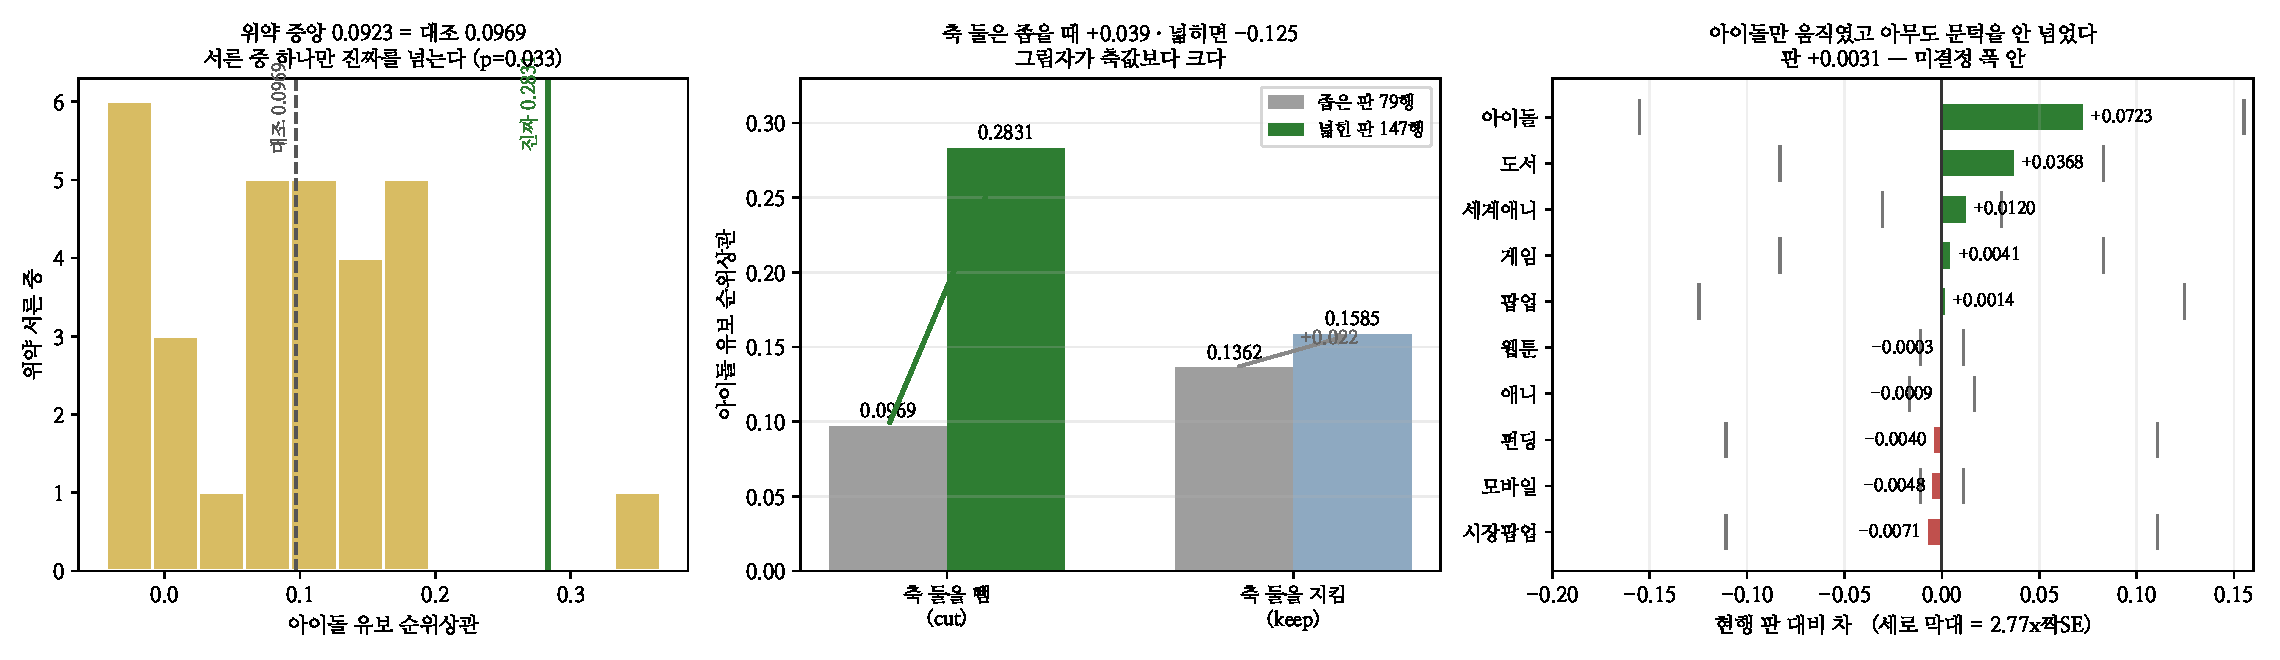
\includegraphics[width=\textwidth]{figs/board.pdf}
\caption{왼쪽 --- 위약 서른의 귀무. 가운데 --- 축$\times$행 $2{\times}2$.
오른쪽 --- 도메인별 현행 대비 차와 문턱.}
\end{figure*}

\section{이겼다 --- 배포 규칙 둘 다 통과}

\begin{center}\footnotesize
\begin{tabular}{lrrr}
\hline
 & 판 & 아이돌 & \\
\hline
현행 \texttt{trendcalwikitag} & 0.3030 & 0.2108 & \\
\textbf{\texttt{idolwide}} & \textbf{0.3061} & \textbf{0.2831} & \\
차 & $+$0.0031 & $+$0.0723 & \\
\hline
\multicolumn{4}{l}{① 판 미결정 폭 0.010 안 --- \textbf{통과}} \\
\multicolumn{4}{l}{② 제일 나쁜 도메인 시장팝업 $-$0.0071 ($t{=}-0.18$)} \\
\multicolumn{4}{l}{\quad 어느 도메인도 $2.77{\times}$짝SE 를 안 넘음 --- \textbf{통과}} \\
\hline
\end{tabular}
\end{center}

덤으로 \textbf{도서가 $+$0.0368} 올랐다 --- 아이돌 학습이 늘면 풀린 계수가
같이 움직이고, 도서는 학습 80행이라 거기에 민감하다(노트 317의 풀링 지도와
같은 자리).

\section{그런데 위약을 서른 번 돌렸다}

\textbf{추가 68행의 라벨만 섞는다.} 행은 그대로 늘어나고 정보만 없앤다.

\begin{center}\small
\begin{tabular}{lr}
\hline
위약 $n{=}30$ 중앙 & 0.0923 \\
\quad 평균 · SD & 0.0869 · \textbf{0.0922} \\
\quad 범위 & [$-$0.0431, \textbf{0.3662}] \\
\hline
같은 경로 대조(\texttt{idolnarrow}) & \textbf{0.0969} \\
위약이 대조 이상인 몫 & \textbf{0.500} \\
\hline
진짜(\texttt{idolwide}) & 0.2831 \\
위약이 진짜 이상인 몫 & \textbf{0.033} ($z{=}2.13$) \\
\hline
\end{tabular}
\end{center}

\paragraph{① 행이 늘어서 버는 몫은 판에서 0 이다} 위약 중앙이 대조와
겹치고 넘는 몫이 정확히 절반이다. 노트 326의 손 부스팅에서는 위약이
$+$0.179 였다 --- 거기서는 학습 54행이 열 피처를 감당 못 해 과적합했고
행이 늘어난 것만으로 나아졌다. \textbf{판은 이미 도메인 열하나를 풀어
쓰므로 그 몫이 없다.} 같은 처치가 작은 판에서는 규제로 일하고 큰 판에서는
정보로만 일한다.

\paragraph{② 이긴 게 맞다, 겨우} 서른 중 하나가 진짜를 넘는다. 그 하나가
0.3662 다 --- \textbf{라벨을 섞었는데 진짜보다 잘 맞힌 판이 있다.}

\paragraph{③ 그리고 이게 제일 크다} 위약의 흩어짐이 \textbf{0.0922} 다.

\begin{center}\small
\begin{tabular}{lrl}
\hline
잡음 & SD & 무엇을 흔드나 \\
\hline
아이돌 짝SE(노트 316) & 0.056 & \textbf{유보 25행} 재추출 \\
\textbf{위약} & \textbf{0.0922} & \textbf{학습 68행}의 라벨 \\
\hline
노트 274 바닥 $2{\times}$짝SE & 0.112 & \\
\textbf{위약 바닥} $2{\times}$SD & \textbf{0.184} & \textbf{1.65배} \\
\hline
오늘의 이득(대조 대비) & 0.1862 & 겨우 넘는다 \\
\hline
\end{tabular}
\end{center}

\textbf{검출 바닥을 유보만 보고 정했던 것이 틀렸다.} 노트 274는 ``같은
자료를 다시 채점하면 얼마나 흔들리나''를 쟀다. 그런데 작은 도메인에서는
\textbf{무엇을 학습에 넣었나가 더 크게 흔든다.} 아이돌은 유보 25 · 학습
122 라 학습 쪽이 다섯 배 크고, 흔들림도 학습 쪽이 크다.

\section{축 둘 --- 노트 326의 한 줄을 고친다}

\begin{center}\footnotesize
\begin{tabular}{lrrr}
\hline
 & 축 둘 뺌 & 축 둘 지킴 & 축값 \\
\hline
좁은 판 79행 & 0.0969 & 0.1362 & \textbf{$+$0.0393} \\
넓힌 판 147행 & \textbf{0.2831} & 0.1585 & \textbf{$-$0.1246} \\
\hline
행값 & $+$0.1862 & $+$0.0223 & \\
\hline
\end{tabular}
\end{center}

노트 326은 ``그 둘은 한터만 쓸 때도 안 벌고 있었다''고 적었다 --- 손
부스팅에서 0.2249 대 0.2199 였다. \textbf{판에서는 $+$0.0393 을 번다.}
고쳐 적는다. \textbf{요점은 축이 쓸모없었다는 게 아니라 그림자가 축값보다
크다는 것이다} --- 넓히는 순간 $+$0.039 가 $-$0.125 로 뒤집힌다.
\textbf{같은 축이 풀에 따라 부호를 바꾼다.}

\section{그리고 아이돌만의 일이 아니다}

\texttt{lab/poolshadow.py} 를 만들어 판이 쓰는 행과 안 쓰는 행의 재료
관측률을 견줬다(\texttt{marker} 와 같은 규약 --- 이름표지 거부권이 아니다).

\begin{center}\footnotesize
\begin{tabular}{lrrl}
\hline
도메인 & 판 & 안 씀 & 풀 모양인 재료 \\
\hline
아이돌 & 79 & 94 & 위키 $+$99\% · 앨범 메타 $+$100\% \\
만화 & 1789 & 611 & 위키 \textbf{$-$39\%} \\
세계애니 & 2948 & 40 & 위키 \textbf{$-$39\%} \\
도서 & 243 & 153 & 검색 $+$80\% \\
\hline
\end{tabular}
\end{center}

\textbf{넷 중 넷이다. 그리고 부호가 다르다.} 아이돌은 \emph{우리가 풀
안쪽만 긁어서} 후보가 비었고, 만화는 \emph{빼 놓은 KR 이 한국어 문서를
더 갖고 있어서} 판 쪽이 비었다. \textbf{원인이 셋인데 결과가 하나다} ---
풀 결정은 언제나 축 결측에 새겨지고, 그 무늬는 필터를 만든 날에는 안 보인다.
부호가 다음 수를 정한다: 후보가 비면 \emph{긁어라}, 판이 비면 \emph{판이
더 가난한 표본이다}.

\section{남은 것}
\begin{center}\footnotesize
\begin{tabular}{ll}
\hline
갈래 & 왜 \\
\hline
\textbf{위약 바닥을 전 도메인에} & 274의 바닥이 다 낮게 잡혔을 수 있다 \\
아이돌 94행 위키 · 앨범 & 축 둘을 되살리는 유일한 길 \\
\texttt{idolwide} 를 승격할까 & $p{=}0.033$ 하나로 자료를 바꿀까 \\
도서가 왜 $+$0.037 인가 & 아이돌을 늘렸는데 도서가 오른다 \\
\hline
\end{tabular}
\end{center}

\paragraph{규약} \textbf{바닥은 유보로만 재는 게 아니다.} 노트 274가
``차가 $2{\times}$짝SE 보다 작으면 못 가른다''를 세웠고 그 뒤 쉰 노트가 그
자로 쟀다. 오늘 위약 서른이 \textbf{학습 쪽 흔들림이 1.65배}라고 알려
줬다. \textbf{작은 도메인에서 우리가 견준 것들 중 일부는 바닥 아래였을 수
있다.} 그리고 이번 이득은 그 바닥을 0.0022 넘겼다 --- \textbf{이겼다고
쓰되, 얼마나 겨우인지도 같이 쓴다.}

\end{document}
